\documentclass[11pt,aspectratio=169]{beamer}

\PassOptionsToPackage{table}{xcolor}
\usetheme{metropolis}
\usepackage{amsmath,amssymb,amsfonts,bm,mathtools}
\usepackage{booktabs,multirow,array}
\usepackage{tikz}
\usetikzlibrary{arrows.meta,positioning,calc,fit,shapes.geometric,decorations.pathreplacing}
\usepackage{graphicx}
\usepackage{xcolor}
\usepackage{colortbl}
\usepackage{pifont}

% ===== Palette =====
\definecolor{cb}{HTML}{1f77b4}\definecolor{cr}{HTML}{d62728}
\definecolor{cg}{HTML}{2ca02c}\definecolor{cy}{HTML}{ff9f00}
\definecolor{cv}{HTML}{9467bd}\definecolor{cgray}{HTML}{555555}
\setbeamercolor{frametitle}{bg=cb!85!black,fg=white}
\setbeamercolor{progress bar}{fg=cb}
\setbeamercolor{alerted text}{fg=cr}

% ===== Math shorthands =====
\newcommand{\R}{\mathbb{R}}
\newcommand{\E}{\mathbb{E}}
\newcommand{\Prb}{\mathbb{P}}
\newcommand{\argmax}{\operatorname*{arg\,max}}
\newcommand{\bel}{\mathbf{b}}
\newcommand{\state}{\mathcal{S}}
\renewcommand{\action}{\mathcal{A}}
\newcommand{\Obs}{\mathcal{O}}

% ===== TikZ shape library =====
\tikzset{
  chance/.style={ellipse,draw,fill=cb!15,minimum width=18mm,minimum height=10mm,thick,inner sep=1pt,font=\footnotesize},
  decision/.style={diamond,draw,fill=cg!18,minimum width=10mm,minimum height=8mm,thick,inner sep=-2pt,aspect=1.6,font=\footnotesize},
  utility/.style={trapezium,trapezium left angle=70,trapezium right angle=110,draw,fill=cy!25,minimum width=12mm,minimum height=9mm,thick,inner sep=2pt,font=\footnotesize},
  state/.style={circle,draw,fill=cb!15,minimum size=10mm,thick,inner sep=1pt,font=\footnotesize\bfseries},
  data/.style={cylinder,draw,shape border rotate=90,aspect=0.25,fill=gray!12,thick,minimum height=8mm,minimum width=18mm,font=\footnotesize},
  hook/.style={fill=cb!10,draw=cb!50,thick,rounded corners=6pt,inner sep=10pt},
  callout/.style={fill=cy!18,draw=cy!60!black,thick,rounded corners=4pt,inner sep=8pt},
  punchline/.style={fill=cr!10,draw=cr!50,very thick,rounded corners=6pt,inner sep=10pt},
  winner/.style={fill=cg!15,draw=cg!50!black,thick,rounded corners=4pt,inner sep=8pt},
}

\setbeamertemplate{frametitle}[default][center]

% ===== Title =====
\title{\textbf{Regime-Switching Asset Allocation via a POMDP}}
\subtitle{\normalsize\textit{Negative headline, decomposed in three diagnostic experiments}}
\author{Dario Blanco Morales \and Even Hogberget \\ Kyle D. Ledda-Lewaren \and Taka Khoo}
\institute{\footnotesize ENGS 177, Decision Making Under Uncertainty\\ \footnotesize Thayer School of Engineering, Dartmouth College}
\date{\footnotesize May 2026}

\begin{document}

% ========== 1. TITLE ==========
\begin{frame}\titlepage\end{frame}

% ========== 2. THE HOOK ==========
\begin{frame}{Have you ever wondered\ldots}
\begin{center}\bigskip
{\Large \emph{Why does the ``safe'' 60/40 portfolio}}\\
{\Large \emph{sometimes lose money when you most need it not to?}}

\bigskip
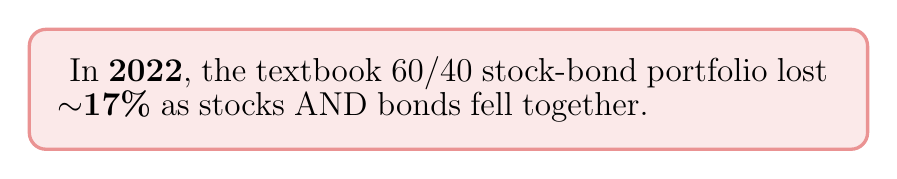
\begin{tikzpicture}
\node[punchline,text width=0.82\textwidth]{\large\centering
  In \textbf{2022}, the textbook 60/40 stock-bond portfolio lost\\
  \textbf{$\sim$17\%} as stocks AND bonds fell together.
};
\end{tikzpicture}

\bigskip
\begin{itemize}\setlength{\itemsep}{4pt}
  \item Static allocation assumes joint return distribution is stable. Reality: conditional heteroskedasticity + stress correlation.
  \item \alert{Question.} Can a fully decision-theoretic regime overlay beat 60/40 out-of-sample after realistic transaction costs?
\end{itemize}
\end{center}
\end{frame}

% ========== 3. ANALOGY: THE DOCTOR ==========
\begin{frame}{The doctor analogy (= POMDP)}
\begin{columns}[T]
\begin{column}{0.58\textwidth}
You are a doctor. Your patient is the market.

\bigskip
\begin{itemize}\setlength{\itemsep}{4pt}
  \item Patient is \emph{healthy} (bull) or \emph{sick} (bear), but you can't examine directly.
  \item You only see symptoms (VIX, term spread, stress indices).
  \item Different treatments (portfolio weights) work better in different states.
  \item Goal: \alert{read symptoms, infer state, prescribe.}
\end{itemize}

\bigskip
\small This IS a POMDP: $s_t$ = regime, $\mathbf{o}_t$ = obs, $\mathbf{a}_t$ = weights, $R$ = expected utility.
\end{column}
\begin{column}{0.40\textwidth}\centering
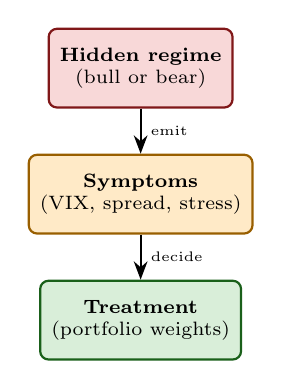
\begin{tikzpicture}[>=Stealth,thick,
    box/.style={rectangle,rounded corners=3pt,draw,thick,minimum width=22mm,minimum height=10mm,inner sep=4pt,font=\scriptsize\bfseries,align=center},
    hidden/.style={box,fill=cr!18,draw=cr!60!black},
    obs/.style={box,fill=cy!22,draw=cy!60!black},
    act/.style={box,fill=cg!18,draw=cg!60!black},
  ]
  \node[hidden] (s) at (0, 2) {Hidden regime\\\scriptsize\mdseries(bull or bear)};
  \node[obs]    (o) at (0, 0.4) {Symptoms\\\scriptsize\mdseries(VIX, spread, stress)};
  \node[act]    (a) at (0, -1.2) {Treatment\\\scriptsize\mdseries(portfolio weights)};
  \draw[->,thick] (s) -- (o) node[midway,right,font=\tiny]{emit};
  \draw[->,thick] (o) -- (a) node[midway,right,font=\tiny]{decide};
\end{tikzpicture}

\bigskip
\footnotesize\textit{Tree, MDP, ID all fail here.}\\
\textit{POMDP is the minimum tool.}
\end{column}
\end{columns}
\end{frame}

% ========== 4. THE PIPELINE ==========
\begin{frame}{End-to-end pipeline}
\vspace{-3mm}
\begin{center}
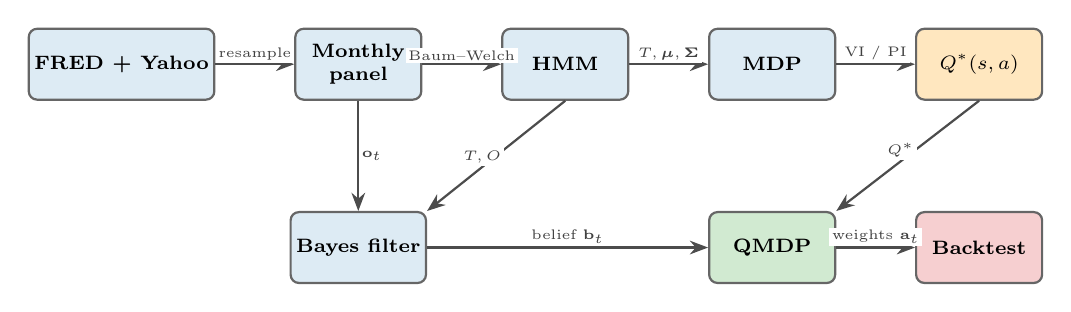
\begin{tikzpicture}[
  node distance=7mm and 10mm,>=Stealth,thick,
  box/.style={rectangle,rounded corners=3pt,draw=black!60,fill=cb!15,thick,minimum width=16mm,minimum height=9mm,inner sep=2pt,font=\scriptsize\bfseries,align=center},
  edge/.style={->,thick,black!70},
  elabel/.style={font=\tiny,color=black!75,fill=white,inner sep=1pt}
]
  % Top row -- all uniform boxes
  \node[box] (raw)                          {FRED + Yahoo};
  \node[box,right=of raw]    (panel)        {Monthly\\panel};
  \node[box,right=of panel]  (hmm)          {HMM};
  \node[box,right=of hmm]    (mdp)          {MDP};
  \node[box,fill=cy!25,right=of mdp] (q)    {$Q^\ast(s,a)$};

  % Bottom row -- below
  \node[box,below=14mm of panel] (filter)   {Bayes filter};
  \node[box,fill=cg!22,below=14mm of mdp] (qmdp) {QMDP};
  \node[box,fill=cr!22,below=14mm of q]   (back) {Backtest};

  % Top row arrows
  \draw[edge] (raw)   -- (panel) node[midway,above,elabel]{resample};
  \draw[edge] (panel) -- (hmm)   node[midway,above,elabel]{Baum--Welch};
  \draw[edge] (hmm)   -- (mdp)   node[midway,above,elabel]{$T,\bm{\mu},\bm{\Sigma}$};
  \draw[edge] (mdp)   -- (q)     node[midway,above,elabel]{VI / PI};

  % Cross-row arrows
  \draw[edge] (panel.south) -- (filter.north) node[midway,right,elabel]{$\mathbf{o}_t$};
  \draw[edge] (hmm.south) -- (filter.north east) node[pos=0.6,above,elabel]{$T,O$};
  \draw[edge] (q.south)   -- (qmdp.north east) node[pos=0.55,above,elabel]{$Q^\ast$};

  % Bottom row arrows
  \draw[edge] (filter) -- (qmdp)  node[midway,above,elabel]{belief $\bel_t$};
  \draw[edge] (qmdp)   -- (back)  node[midway,above,elabel]{weights $\mathbf{a}_t$};
\end{tikzpicture}
\end{center}

\vspace{-2mm}
\footnotesize
\begin{itemize}\setlength{\itemsep}{2pt}
  \item \textbf{Top (offline, do once):} fit HMM, solve MDP, build $Q^\ast$. VI and PI agree to $2.6\!\times\!10^{-6}$.
  \item \textbf{Bottom (each month):} new observation $\to$ updated belief $\to$ QMDP $\to$ weights $\to$ realised return.
  \item \textbf{Walk-forward} 2003-10 $\to$ 2026-04, monthly rebalance, 5\,bps tx cost, 271 decisions.
\end{itemize}
\end{frame}

% ========== 5. QMDP RULE + WORKED EXAMPLE ==========
\begin{frame}{QMDP rule, with a worked example}
\[
\boxed{\pi_{\rm QMDP}(\mathbf{b}) = \argmax_{\mathbf{a}} \sum_s b(s)\,Q^\ast(s, \mathbf{a})}
\]

\smallskip
\textbf{Decision moment.} After a VIX spike the belief filter returns $\bel=(0.07,\,0.93)$ (bear-leaning). At the \emph{headline} $\gamma{=}2$, the $Q^\ast$ table is genuinely regime-differentiated:

\centering\small\renewcommand{\arraystretch}{1.1}
\begin{tabular}{l rr r}
\toprule
\textbf{Action} & $Q^\ast(\text{bull})$ & $Q^\ast(\text{bear})$ & $\bel^\top Q^\ast(\cdot,\mathbf{a})$ \\
\midrule
100/0 stocks       & 0.183 & 0.024 & 0.035 \\
60/40              & 0.180 & 0.028 & 0.038 \\
\rowcolor{cg!20}\textbf{0/100 bonds} & 0.174 & 0.032 & \textbf{0.042} \\
\bottomrule
\end{tabular}

\smallskip\small Bull column rewards stocks (argmax $=100/0$); bear column rewards bonds (argmax $=0/100$). The bear-leaning belief makes QMDP pick \alert{0/100}: a genuine regime-driven decision at the canonical $\gamma{=}2$.
\end{frame}

% ========== 6. THE HORSE RACE ==========
\begin{frame}{Twelve-strategy horse race (2003--2026, 5\,bps cost)}
\centering\scriptsize\setlength{\tabcolsep}{4pt}\renewcommand{\arraystretch}{1.05}
\begin{tabular}{l rrrrrr}
\toprule
\textbf{Strategy} & \textbf{CAGR} & \textbf{Vol} & \textbf{Sharpe} & \textbf{Sortino} & \textbf{Max DD} & \textbf{Calmar} \\
\midrule
\rowcolor{cg!20}\textbf{Faber 10-mo SMA} & \textbf{17.24\%} & 9.80\%  & \textbf{1.68} & \textbf{3.57} & $-13.5\%$ & \textbf{1.28} \\
Myopic 12-mo trend                       & 15.34\% & 10.57\% & 1.41 & 2.70 & $-15.1\%$ & 1.01 \\
TS momentum 12-mo                        & 9.06\%  & 8.25\%  & 1.10 & 1.74 & $-22.0\%$ & 0.41 \\
HMM-conditional MV                       & 6.38\%  & 5.91\%  & 1.08 & 1.78 & $-18.4\%$ & 0.35 \\
Black--Litterman + HMM                   & 6.17\%  & 6.65\%  & 0.94 & 1.45 & $-18.0\%$ & 0.34 \\
Inverse-vol                              & 4.78\%  & 5.24\%  & 0.92 & 1.42 & $-16.8\%$ & 0.28 \\
Risk parity (ERC)                        & 4.87\%  & 5.37\%  & 0.91 & 1.41 & $-16.8\%$ & 0.29 \\
Equal weight 50/50                       & 6.69\%  & 8.12\%  & 0.84 & 1.26 & $-28.6\%$ & 0.23 \\
Mean-variance + Ledoit-Wolf              & 6.58\%  & 8.20\%  & 0.82 & 1.32 & $-22.5\%$ & 0.29 \\
Static 60/40 (benchmark)                 & 7.40\%  & 9.35\%  & 0.81 & 1.21 & $-34.2\%$ & 0.22 \\
Vol-target 60/40                         & 7.50\%  & 10.14\% & 0.77 & 1.12 & $-39.1\%$ & 0.19 \\
\rowcolor{cr!18}\textbf{QMDP ($\gamma{=}2$)} & 10.01\% & 14.64\% & \textbf{0.73} & 1.07 & $\mathbf{-53.0\%}$ & 0.19 \\
\bottomrule
\end{tabular}

\bigskip\small
\textbf{Three sentences.} (1) Faber dominates every metric. (2) \alert{QMDP is dead last on Sharpe} with the deepest drawdown. (3) HMM-aware non-QMDP baselines (HMM-MV, BL+HMM) beat QMDP $\Rightarrow$ the HMM signal IS informative.
\end{frame}

% ========== 7. EQUITY CURVES FIGURE ==========
\begin{frame}{Equity curves: \$1 invested 2003-10-31 (log scale)}
\centering
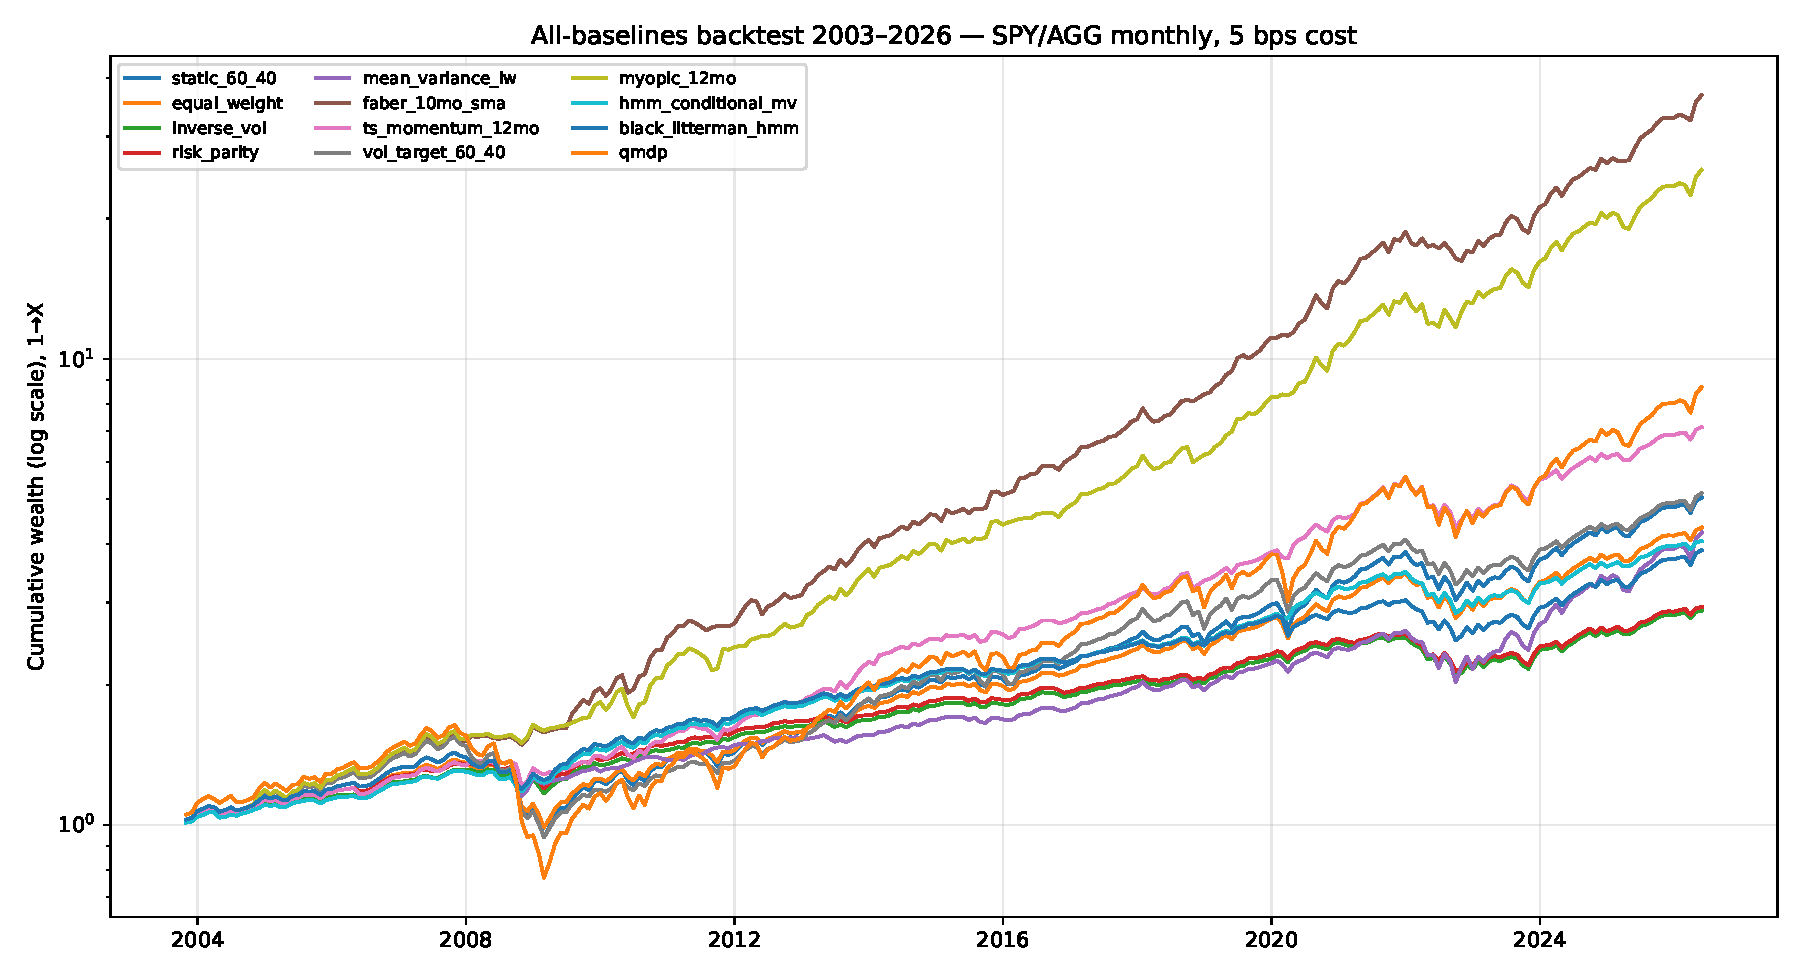
\includegraphics[height=0.78\textheight,keepaspectratio]{../figures/baselines_equity.pdf}

\smallskip\scriptsize Faber (top) ends near \$30. QMDP (red) ends near \$8 with the deepest mid-figure trench. Static 60/40 ends near \$5.
\end{frame}

% ========== 8. THE GAMMA COLLAPSE ==========
\begin{frame}{Why QMDP collapsed: regime label never moves the policy}
\centering\small\setlength{\tabcolsep}{8pt}\renewcommand{\arraystretch}{1.2}
\begin{tabular}{lccccccc}
\toprule
\textbf{Regime} & $\gamma{=}1$ & $\gamma{=}2$ & $\gamma{=}3$ & $\gamma{=}5$ & $\gamma{=}8$ & $\gamma{=}15$ & $\gamma{=}20$ \\
\midrule
Bull (0) & 100/0 & 100/0 & 100/0 & 80/20 & 40/60 & 20/80 & 20/80 \\
Bear (1) & 100/0 & 100/0 & 100/0 & 80/20 & 40/60 & 20/80 & 20/80 \\
\bottomrule
\end{tabular}

\bigskip
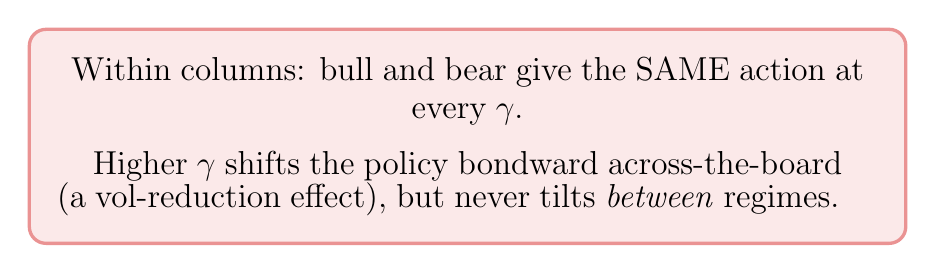
\begin{tikzpicture}
\node[punchline,text width=0.86\textwidth]{\centering
  \large \alert{Within columns:} bull and bear give the SAME action at every $\gamma$.\\
  \medskip
  Higher $\gamma$ shifts the policy bondward across-the-board\\
  (a vol-reduction effect), but never tilts \emph{between} regimes.
};
\end{tikzpicture}

\bigskip\small A low-$\gamma$ ``gambler'' bets the same way regardless of suspicion. Only $\gamma \geq 8$ would let suspicion shift the policy, and even then, both regimes shift together.
\end{frame}

% ========== 9. UNLOCK 1 TABLE ==========
\begin{frame}{Unlock 1: richer observations FIX the policy at $\gamma{=}2$}
\centering\small\setlength{\tabcolsep}{6pt}\renewcommand{\arraystretch}{1.2}
\begin{tabular}{l l cc c}
\toprule
\textbf{Cohort} & \textbf{Features} & \textbf{Bull} & \textbf{Bear} & \textbf{Differs?} \\
\midrule
1. Baseline         & VIX, T10Y3M             & 100/0 & 100/0 & \ding{55} \\
2. +Yield curve     & +T10Y2Y                 & 100/0 & 100/0 & \ding{55} \\
\rowcolor{cg!20}\textbf{3. +Stress} & \textbf{+NFCI, +STLFSI4} & \textbf{100/0} & \textbf{0/100} & \textbf{\ding{51}\ full flip} \\
4. +Macro           & +UMCSENT, +ICSA         & 100/0 & 0/100 & \ding{51} \\
5. Kitchen sink     & 8 channels              & 100/0 & 60/40 & \ding{51} \\
\bottomrule
\end{tabular}

\bigskip
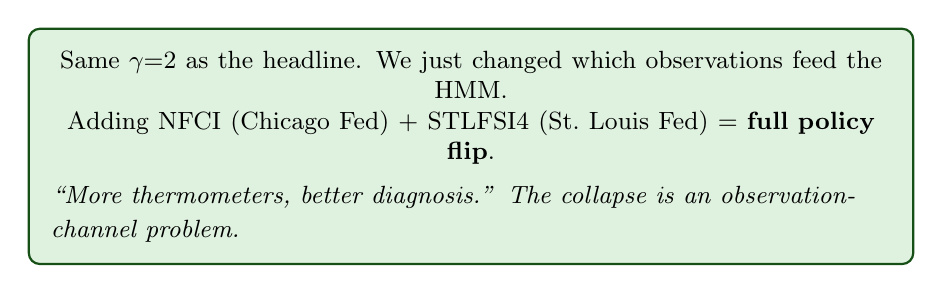
\begin{tikzpicture}
\node[winner,text width=0.88\textwidth]{\centering\small
  Same $\gamma{=}2$ as the headline. We just changed which observations feed the HMM.\\
  Adding \alert{NFCI} (Chicago Fed) + \alert{STLFSI4} (St.\ Louis Fed) = \textbf{full policy flip}.\\[4pt]
  \emph{``More thermometers, better diagnosis.'' The collapse is an observation-channel problem.}
};
\end{tikzpicture}
\end{frame}

% ========== 10. UNLOCK 1 VISUAL ==========
\begin{frame}{Visual confirmation of Unlock 1}
\centering
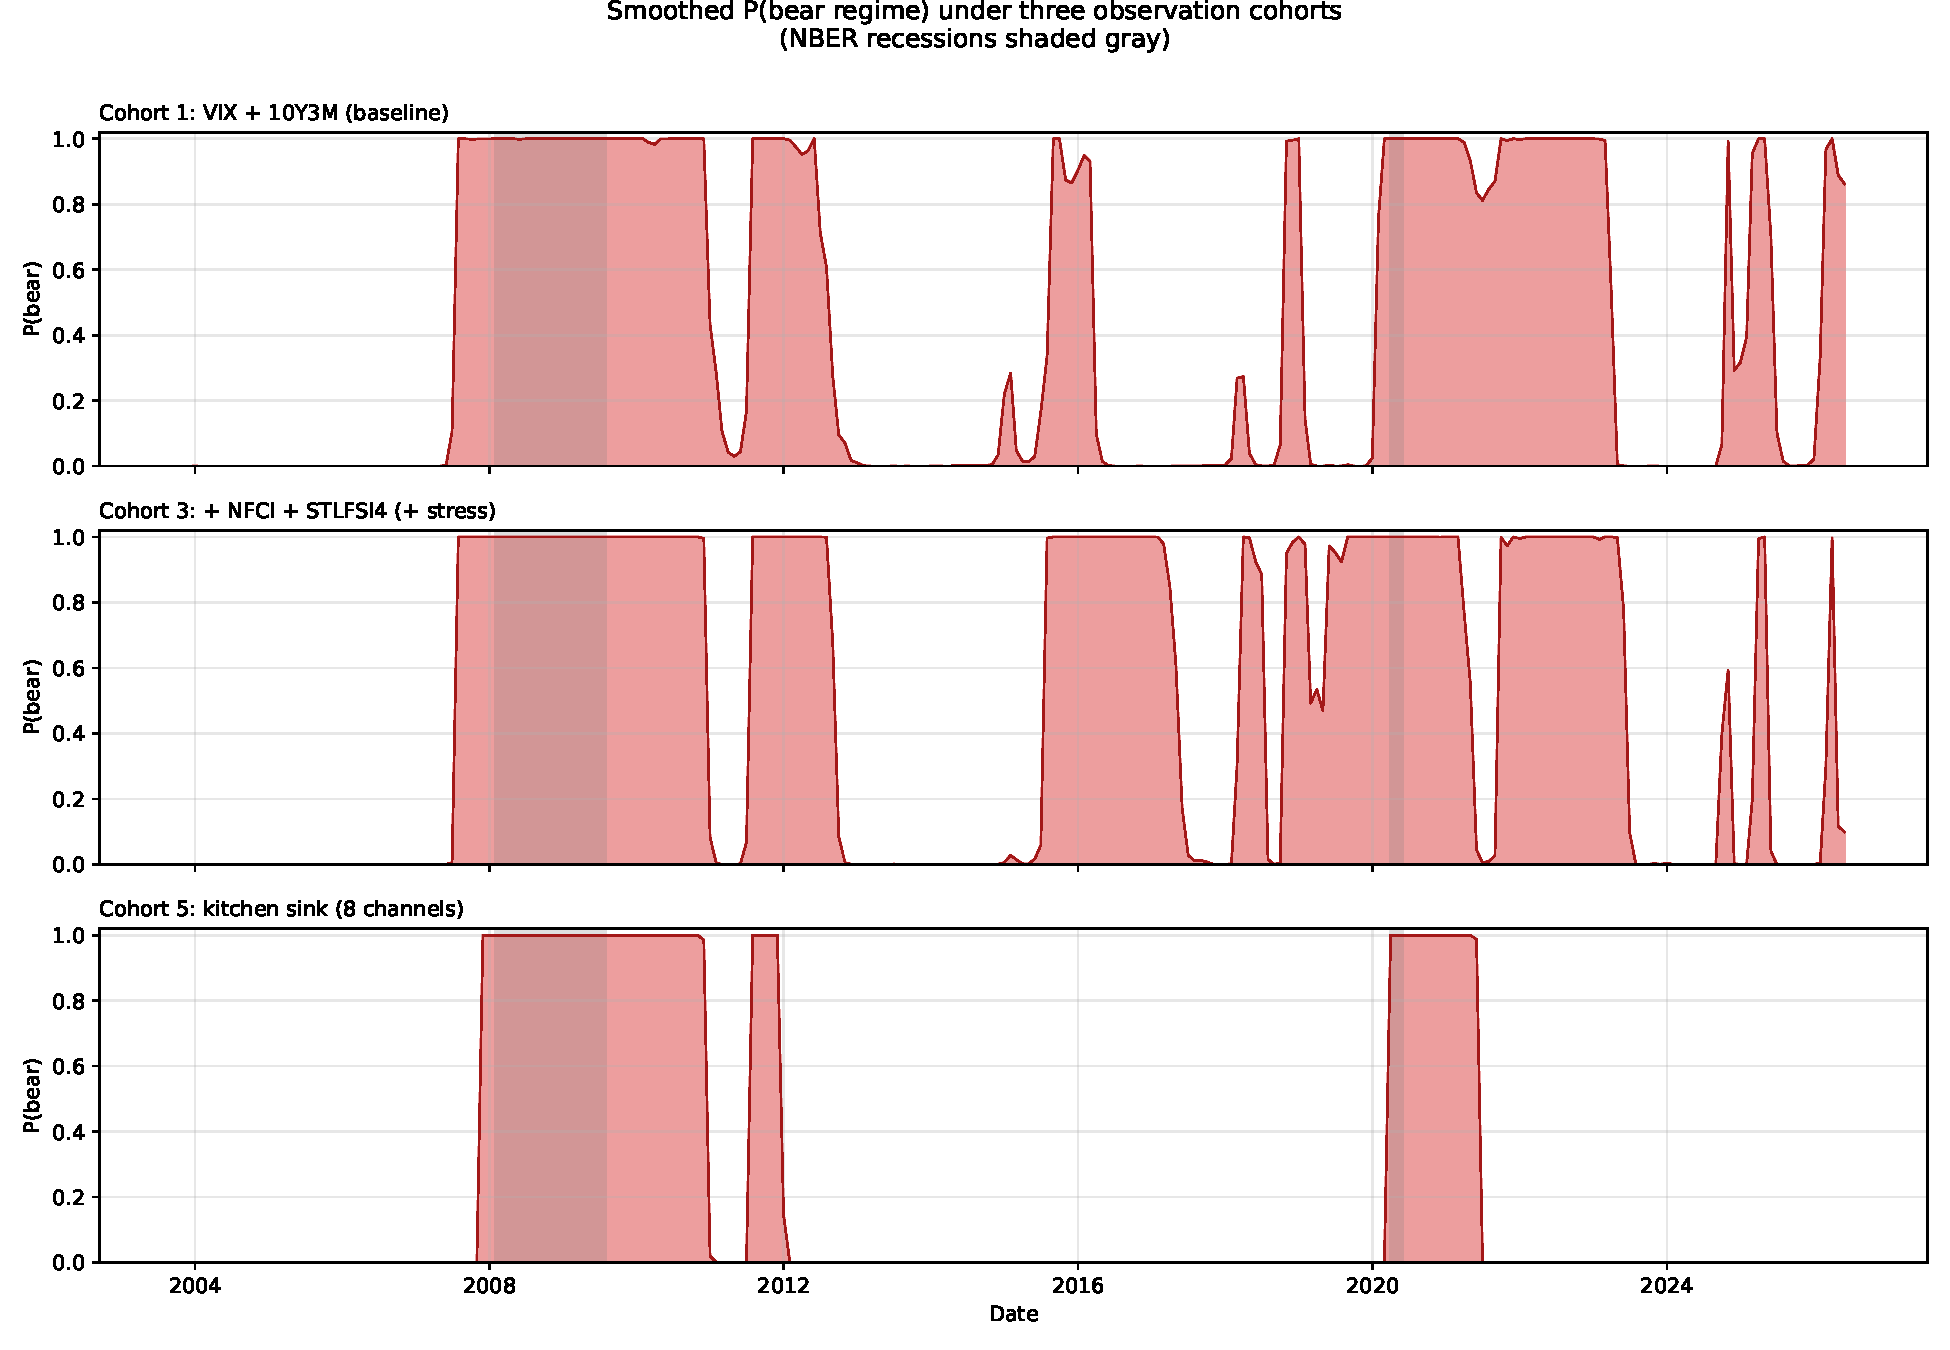
\includegraphics[height=0.74\textheight,keepaspectratio]{../figures/cohort_regime_timelines.pdf}

\smallskip\scriptsize Top: cohort 1 (baseline, noisy false alarms). \alert{Middle: cohort 3 (+NFCI, +STLFSI4), with sharp bear spikes cleanly bracketing every NBER recession.} Bottom: cohort 5 (kitchen sink, over-fits).
\end{frame}

% ========== 11. UNLOCK 2 TABLE ==========
\begin{frame}{Unlock 2: walk-forward refit lifts Sharpe to 1.08}
\centering\small\setlength{\tabcolsep}{8pt}\renewcommand{\arraystretch}{1.2}
\begin{tabular}{l rrrr}
\toprule
\textbf{Variant} & \textbf{CAGR} & \textbf{Sharpe} & \textbf{Max DD} & \textbf{Calmar} \\
\midrule
Static 60/40 (benchmark)     & 7.40\% & 0.81 & $-34.2\%$ & 0.22 \\
QMDP fixed (report baseline) & 9.87\% & 0.96 & $-34.2\%$ & 0.29 \\
QMDP annual refit (5y win)   & 9.11\% & 0.85 & $-25.1\%$ & 0.36 \\
QMDP quarterly refit         & 8.56\% & 0.83 & $-23.4\%$ & 0.37 \\
\rowcolor{cg!20}\textbf{QMDP expanding window} & 9.81\% & \textbf{1.08} & $\mathbf{-16.5\%}$ & \textbf{0.60} \\
HMM-MV expanding window      & 5.32\% & 0.95 & $-16.8\%$ & 0.32 \\
\bottomrule
\end{tabular}

\bigskip
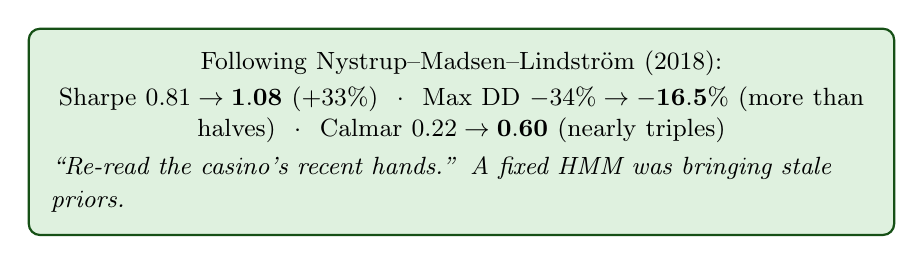
\begin{tikzpicture}
\node[winner,text width=0.86\textwidth]{\centering\small
  Following Nystrup--Madsen--Lindstr\"om (2018):\\[2pt]
  \alert{Sharpe} $0.81 \to \mathbf{1.08}$ (+33\%)\ \ $\cdot$\ \ \alert{Max DD} $-34\% \to \mathbf{-16.5\%}$ (more than halves)\ \ $\cdot$\ \ \alert{Calmar} $0.22 \to \mathbf{0.60}$ (nearly triples)\\[2pt]
  \emph{``Re-read the casino's recent hands.'' A fixed HMM was bringing stale priors.}
};
\end{tikzpicture}
\end{frame}

% ========== 12. SUBPERIOD HEATMAP ==========
\begin{frame}{Subperiod robustness: QMDP fails worst where it should help}
\centering
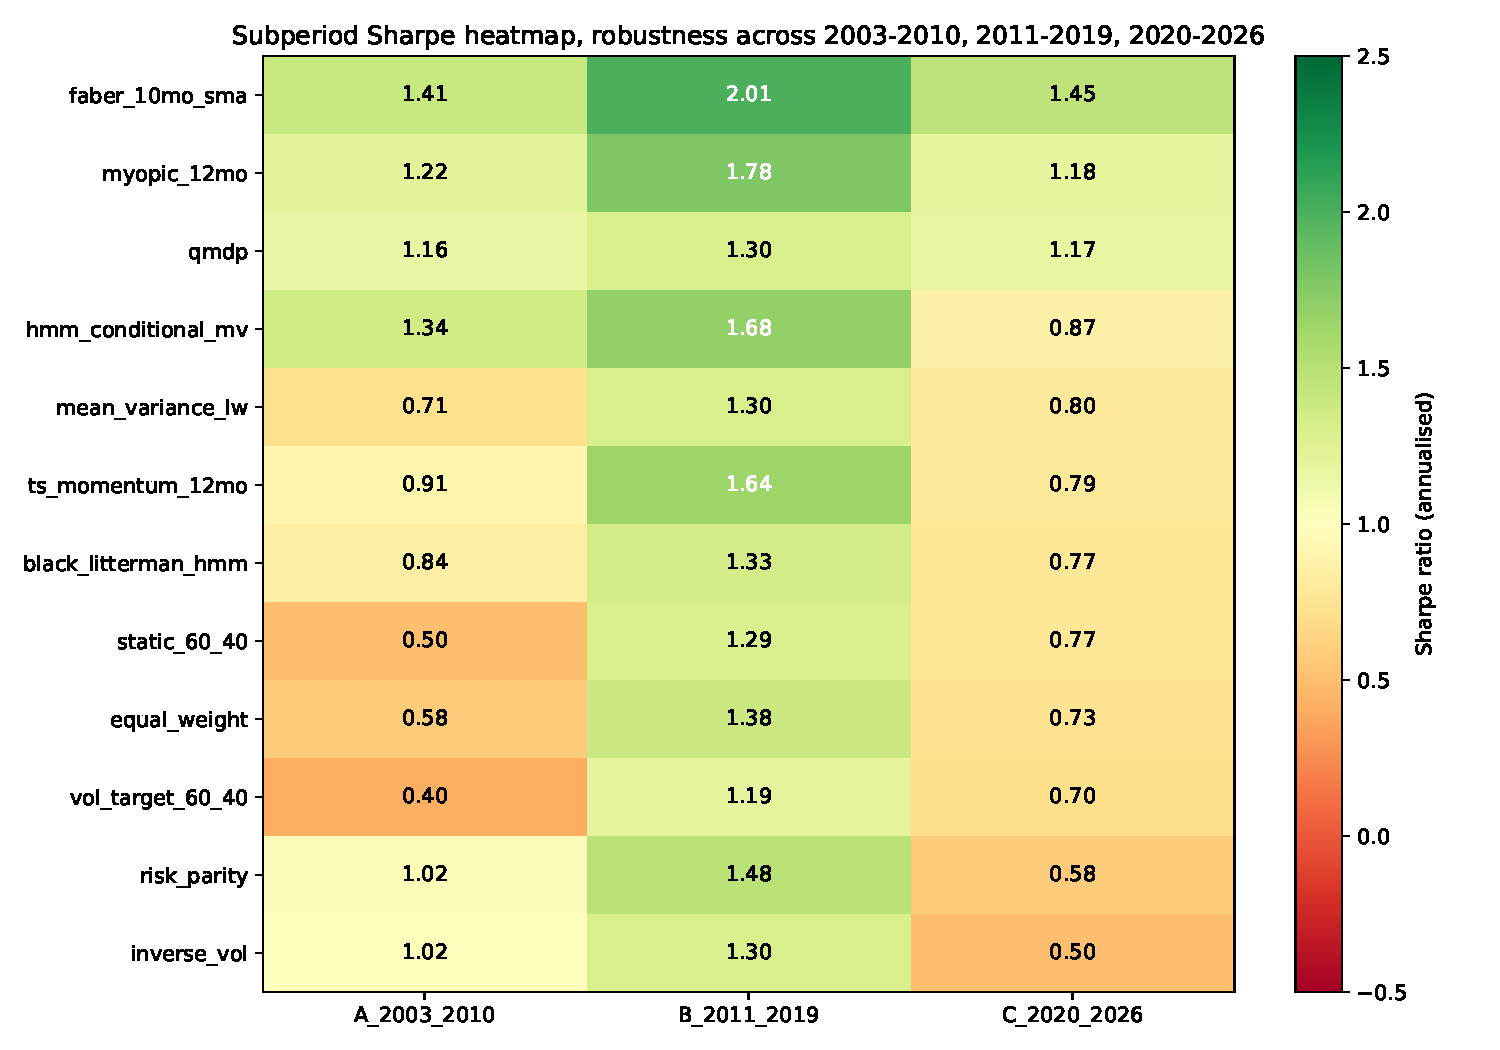
\includegraphics[height=0.55\textheight,keepaspectratio]{../figures/subperiod_sharpe_heatmap.pdf}

\vspace{2pt}\footnotesize
\begin{itemize}\setlength{\itemsep}{0pt}
  \item \textbf{Faber dominates every column.} The trend rule isn't a one-period fluke.
  \item \alert{QMDP's worst column is Period~A (GFC, Sharpe 0.33)}: exactly where a regime model should help most.
  \item In the same Period~A, HMM-MV and BL+HMM (same signal, no QMDP projection) get Sharpe \textbf{1.03--1.25} $\Rightarrow$ \textbf{QMDP's $\gamma{=}2$ projection destroyed it.}
\end{itemize}
\end{frame}

% ========== 13. THE HONEST VERDICT ==========
\begin{frame}{The honest verdict: claim vs.\ non-claim}
\centering\small\renewcommand{\arraystretch}{1.4}
\begin{tabular}{|>{\columncolor{cg!10}}p{0.46\textwidth}|>{\columncolor{cr!8}}p{0.46\textwidth}|}
\hline
\textbf{We DO claim} & \textbf{We do NOT claim} \\
\hline
POMDP is the right \emph{minimum} tool for this decision problem. & POMDP asset allocation beats simple trend-following. \\
\hline
The headline negative finding is a diagnostic of methodology, not fundamentals. & The original QMDP at $\gamma{=}2$ is a useful production policy. \\
\hline
The HMM signal is informative (HMM-MV, BL+HMM beat QMDP). & Our walk-forward QMDP is the new state-of-the-art. \\
\hline
Three components separately reverse the negative finding: observations, refit, $\gamma$. & Our gains net of transaction costs matter to a real allocator. \\
\hline
\end{tabular}

\bigskip\small
\textit{Negative-with-decomposition} is more useful than a positive headline. The diagnostic table outlasts any specific sample's Sharpe number.
\end{frame}

% ========== 14. EXTENSIONS ==========
\begin{frame}{Three extensions in priority order}
\bigskip
\begin{enumerate}\setlength{\itemsep}{14pt}
  \item \alert{CVaR-penalised reward.}\\
        \small Replace CRRA utility with $R = \E[r] - \kappa\,\mathrm{CVaR}_\alpha[r]$ to explicitly penalise bear-regime tail risk. One-line change in the reward function.

  \item \alert{Point-based value iteration (PBVI).}\\
        \small Maintain explicit $\alpha$-vectors over a small set of reachable beliefs. Gives a tighter upper bound on QMDP. On a 1-D belief simplex the cost is negligible.

  \item \alert{Off-policy MC + Double Q-learning.}\\
        \small A genuinely model-free baseline that does \emph{not} assume the QMDP transition matrix is correct. Cross-checks the model-based pipeline against learning from scratch.
\end{enumerate}
\end{frame}

% ========== 15. THANK YOU ==========
\begin{frame}[plain]
\vspace*{\fill}
\begin{center}
{\Huge\textbf{Thank you.}}\\[18pt]
{\LARGE Questions?}
\end{center}
\vspace*{\fill}
\end{frame}

\end{document}
